\documentclass[hyperref={xetex,colorlinks,linkcolor=blue},green,compress]{beamer}
\usepackage{multicol}
\usepackage{latexsym,pifont,units,amsmath,amsfonts,amssymb}
\usepackage{xltxtra} %fontspec,xunicode are loaded here.
%\usepackage{graphicx} % beamer loads graphicx already.
\graphicspath{{./figs/}{../figs/}{./}{../}} %note that the trailing “/” is required
%\usepackage{pdfsync,comment}
\usepackage{tikz}
\usetikzlibrary{arrows,decorations.pathmorphing,backgrounds,positioning,fit}
\usepackage{listings}
\lstset{language=c, basicstyle=\small, stringstyle=\ttfamily,backgroundcolor=\color{red!10},emph={down,up}, emphstyle=\color{red},numberstyle=\tiny,numbersep=.5em}
\usepackage{xeCJK}

\setsansfont[Mapping=tex-text]{DejaVu Sans}

% \setCJKmainfont[BoldFont={WenQuanYi Zen Hei}, ItalicFont={WenQuanYi Zen Hei}]{SimSun}
% \setCJKfamilyfont{hei}{WenQuanYi Zen Hei}
% \setCJKfamilyfont{song}{SimSun}

%\newcommand{\ziju}[1]{\renewcommand{\CJKglue}{\hskip #1}}
\usetheme{default}
\usecolortheme{rose}
\usefonttheme[onlysmall]{structurebold}
\usenavigationsymbolstemplate{}
\setbeamertemplate{footline}[frame number]
\setbeamertemplate{navigation symbols}{}
\setbeamertemplate{blocks}[rounded][shadow=true]
%\setbeameroption{show notes}
%\beamertemplateballitem

\newcommand\googlelogo{\includegraphics[height=1em]{google}}

\begin{document}
\title{Network Basics} \institute{School of CIS\\SWFU} \author{Wang Xiaolin}

\begin{frame}
  \titlepage \vfill \tiny{\ding{41} wx672ster@gmail.com\\\ding{37} 13577067397}
\end{frame}

% \begin{frame}\frametitle{Outline}
%   \begin{multicols}{2}
%     \tableofcontents
%   \end{multicols}
% \end{frame}

\section{Introduction}
\label{sec:intro}

% \begin{frame}\frametitle{}
%   \begin{multicols}{2}
%     \tableofcontents[currentsection]
%   \end{multicols}
% \end{frame}

\subsection[Definition]{What's A Computer Network?}
\label{sec:whats}

\begin{frame}\frametitle{{What's A Computer Network?}}
  
\begin{itemize}
\item \href{http://en.wikipedia.org/wiki/Computer\_network}{http://en.wikipedia.org/wiki/Computer\_network}
\end{itemize}

\begin{center}
  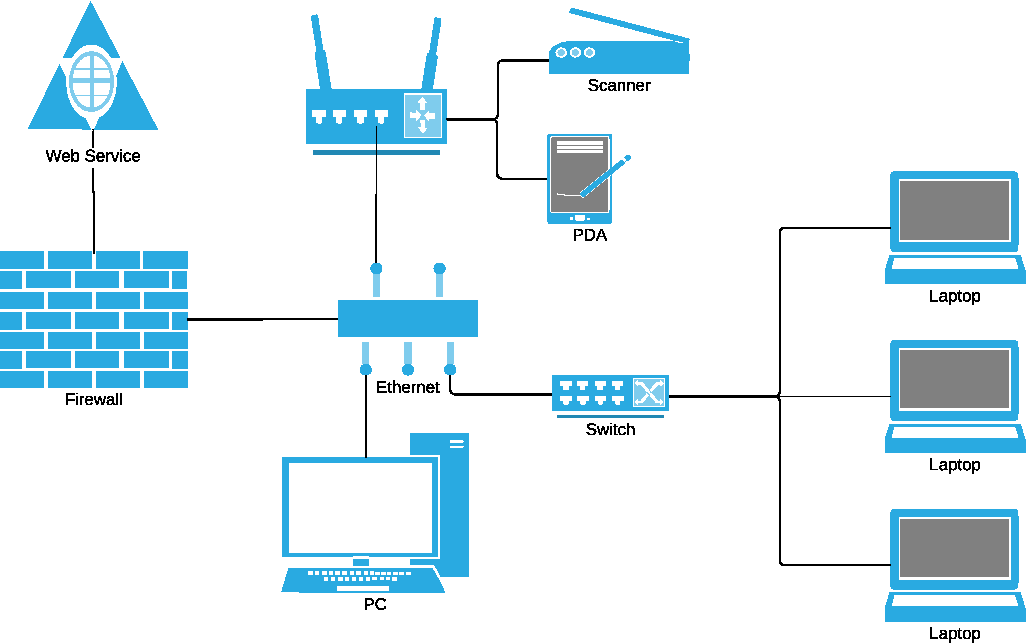
\includegraphics[width=.5\textwidth]{network}
\end{center}

\end{frame}

\subsection[History]{Past and Future}
\label{sec:history}

\begin{frame}\frametitle{The History of Internet}

\begin{tabular}{rl}
  1836:&Telegraph\\
  1858-1866:&Transatlantic cable\\
  1876:&Telephone\\
  1957:&USSR launches Sputnik\\
  1962-1968:&Packet-switching networks developed\\
  1969:&Birth of Internet\\
  1971:&People communicate over a network\\
  1977:&E-mail takes off, Internet becomes a reality\\
  1982:&TCP/IP defines future communication\\
  1987:&Commercialisation of Internet Born\\
  1993:&The WWW Revolution truly begins\\
  1996:&Microsoft enters
\end{tabular}
%1972: Computers can connect more freely and easily
%% 1973: Global Networking becomes a reality
%% 1974: Packets become mode of transfer
%% 1976: Networking comes to many
%% 1979: News Groups born
%% 1981: Things start to come together
%% 1983: Internet gets bigger
%% 1984: Growth of Internet Continues
%% 1986: Power of Internet Realised
%% 1989: Large growth in Internet
%% 1990: Expansion of Internet continues
%% 1991: Modernisation Begins
%% 1992: Multimedia changes the face of the Internet
%% 1994: Commercialisation begins
%% 1995: Commercialisation continues apace
\begin{itemize}
\item \href{http://www.faqs.org/rfcs/rfc2235.html}{RFC2235 --- Hobbes' Internet Timeline}(\href{http://www.zakon.org/robert/internet/timeline/}{v8.2})
\item \href{http://www.netvalley.com/archives/mirrors/davemarsh-timeline-1.htm}{Internet History Timeline}
\end{itemize}
\end{frame}

\subsection[Classification]{Network Classification}
\label{sec:classification}

\begin{frame}\frametitle{Network Classification}

\begin{itemize}
\item connection method: wired, wireless...
\item topology
\item scale
\item network architecture: c/s, p2p...
\end{itemize}

\end{frame}

\begin{frame}\frametitle{Network Classification}\framesubtitle{Connection method}

  Wired Technologies:
\begin{center}
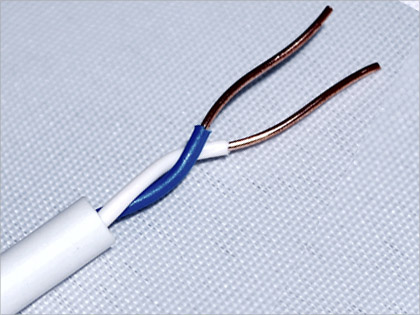
\includegraphics[height=2cm]{twisted-pair}
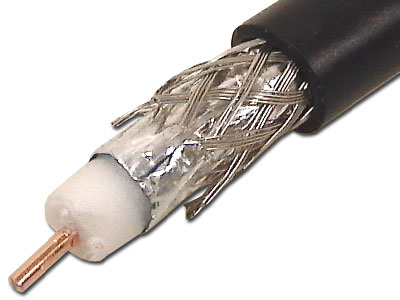
\includegraphics[height=2cm]{coaxial-cable}
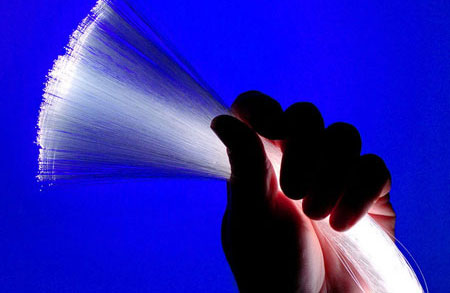
\includegraphics[height=2cm]{fiber-optics}
\end{center}
Wireless Technologies:
\begin{center}
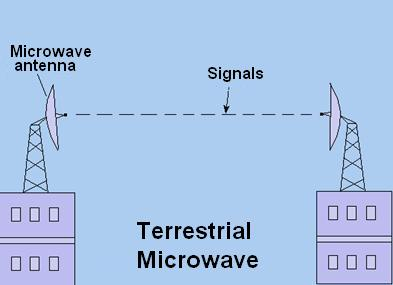
\includegraphics[height=2cm]{terrestrial}
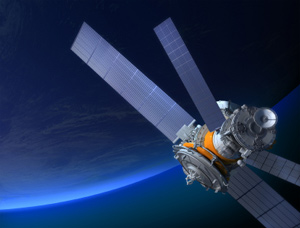
\includegraphics[height=2cm]{satellite}
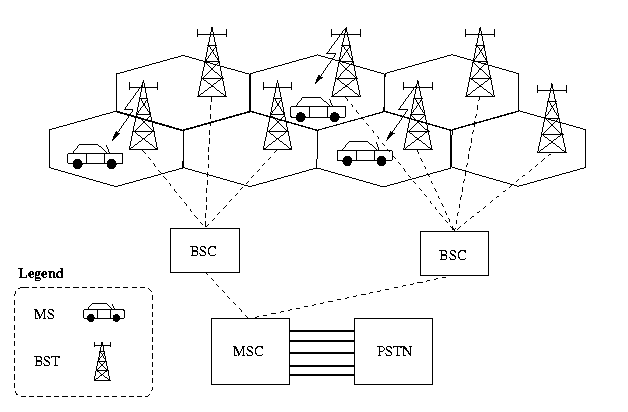
\includegraphics[height=2cm]{cellular}\\
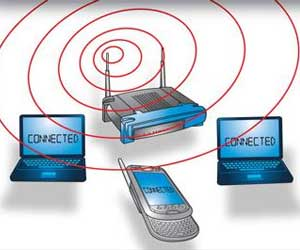
\includegraphics[height=2cm]{wlan}

\includegraphics[height=2cm]{bluz}
\end{center}
\end{frame}

\begin{frame}\frametitle{Network Classification}\framesubtitle{Scale}
\small{PAN}, \large{LAN}, \Large{CAN}, \LARGE{WAN}, \Huge{MAN} ...
\end{frame}

\begin{frame}\frametitle{Network Classification}\framesubtitle{Topology}
  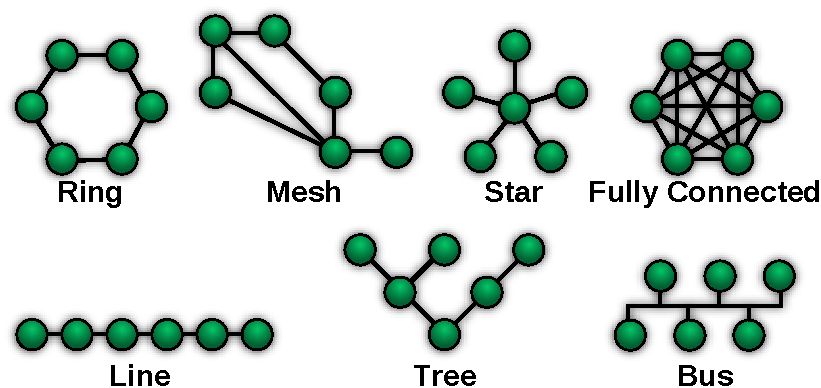
\includegraphics[width=\textwidth]{topo}
\end{frame}

\begin{frame}\frametitle{Network Classification}\framesubtitle{Network Architecture}
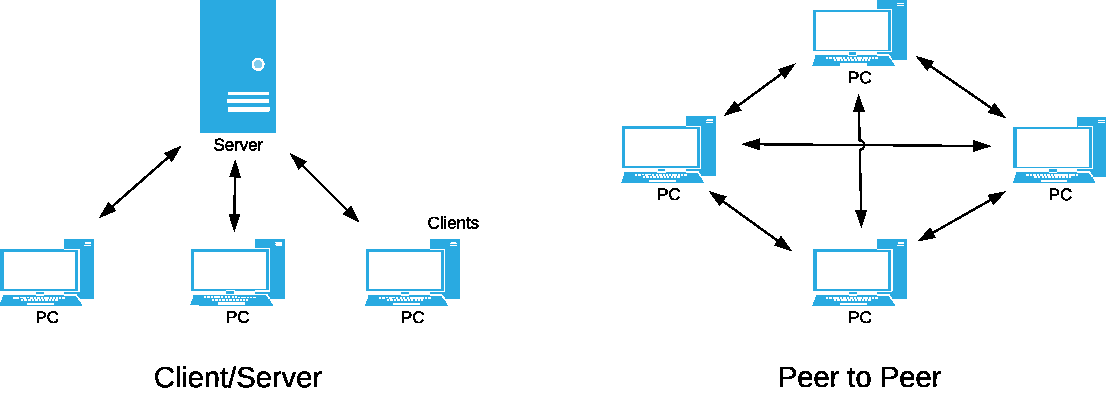
\includegraphics[width=\textwidth]{arch}
\end{frame}

\subsection[Hardwares]{Basic Hardware Components}
\label{sec:hw}

\begin{frame}\frametitle{Basic Hardware Components}
\begin{center}
\begin{tabular}{rl|rl}
 NIC:&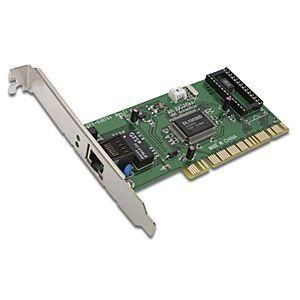
\includegraphics[height=1cm]{nic}&Repeater:&
\includegraphics[height=1cm]{repeater}\\
 Hub:&
\includegraphics[height=1cm]{hub}&Bridge:&
\includegraphics[height=1cm]{bridge}\\
 Switch:&
\includegraphics[height=1cm]{switch}&Router:&
\includegraphics[height=1cm]{router}
\end{tabular}
\end{center}
\end{frame}


\subsection{Applications}
\label{sec:app}

\begin{frame}\frametitle{What Computer Networks For?}
\begin{itemize}
\item Resources sharing
\item communicating
\item more ...
\end{itemize}
\end{frame}

\section{How The Internet Works?}
\label{sec:principle}

% \begin{frame}\frametitle{}
% \small{\tableofcontents[currentsection]}
% \end{frame}

\subsection[Definition]{What's The Internet?}
\label{sec:whatsinternet}

\begin{frame}\frametitle{What's The Internet?}
\begin{itemize}
\item The network of networks.
\item Tech view: \href{http://en.wikipedia.org/wiki/Tcp/ip}{TCP/IP}
\item App view: \href{http://en.wikipedia.org/wiki/Google}{\googlelogo}
\end{itemize}
\end{frame}

\subsection[TCP/IP]{What's TCP/IP?}
\label{sec:tcpip}

\begin{frame}\frametitle{What's TCP/IP?}
A set of communication protocols designed for the Internet.

\begin{description}
\item[what's a protocol?] a rule, a treaty, an agreement ...
\end{description}
\end{frame}

\begin{frame}\frametitle{TCP/IP Protocol Stack}
  Every networked computer has it inside.

\begin{center}
  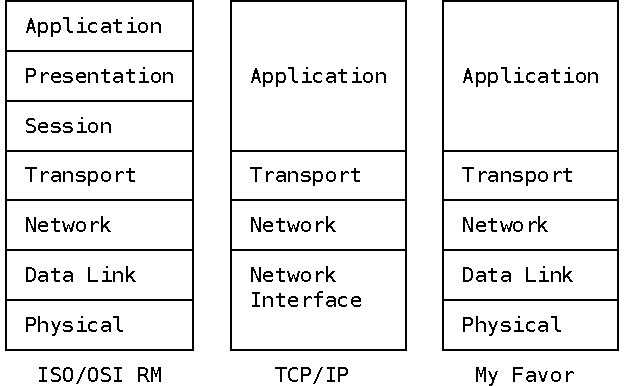
\includegraphics[width=.8\textwidth]{stack}
\end{center}
\end{frame}

  \begin{frame}
    \frametitle{TCP/IP Overview} \framesubtitle{Basic Structure}
    \begin{columns}[t]
      \begin{column}{.5\textwidth}
        \begin{figure}
          \centering
          \includegraphics[width=.95\textwidth]{basic-structure}
          \caption{Basic TCP/IP Network Node}
          \label{fig:basic-node}
        \end{figure}
      \end{column}

      \begin{column}{.5\textwidth}
        
        \begin{exampleblock}{Questions we're going to answer:}
        \begin{enumerate}
        \item Where will an incoming Ethernet frame go? ARP module or IP module?
%          (Figure~\ref{fig:ethernet-frame-format}, 0x0800$/$0x0806)
        \item Where will an incoming IP packet go? UDP module or TCP module? %(Figure~\ref{fig:ip-packet-format}, 17$/$6)
        \item Where will an incoming transport message (UDP datagram, TCP segment) go? TELNET or FTP or ...?
%          (Figure~\ref{fig:udp-datagram-format} and Figure~\ref{fig:tcp-segment-format})
        \end{enumerate}
        \end{exampleblock}
      \end{column}
    \end{columns}
  \end{frame}

  \begin{frame}
    \frametitle{The Name Of A Unit Of Data}
    \begin{columns}
      \begin{column}{.5\textwidth}
        \begin{itemize}
        \item Application Message
        \item TCP Segment %% (Figure~\ref{fig:tcp-segment-format})
          , UDP
          Datagram %% (Figure~\ref{fig:udp-datagram-format})
        \item IP packet (Fig.~\ref{fig:ip-packet-format})
        \item Ethernet frame (Fig.~\ref{fig:ethernet-frame-format})
        \end{itemize}
      \end{column}
      \begin{column}{.5\textwidth}
        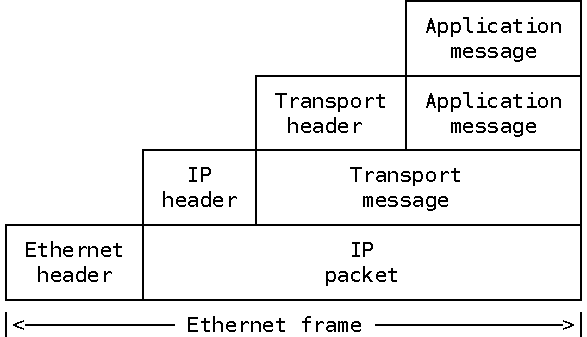
\includegraphics[width=\textwidth]{encap}
      \end{column}
    \end{columns}
  \end{frame}

  \subsubsection{Ethernet}

  \begin{frame}
    \frametitle{Ethernet}
    \begin{enumerate}
    \item Frame format?
    \item Address format?
    \item Broadcast address?
    \item CSMA/CD? (Please explain)
    \end{enumerate}
  \end{frame}

  \begin{frame}
    \frametitle{Ethernet} \framesubtitle{Ethernet Version II Frame}
    \begin{figure}
      \centering
      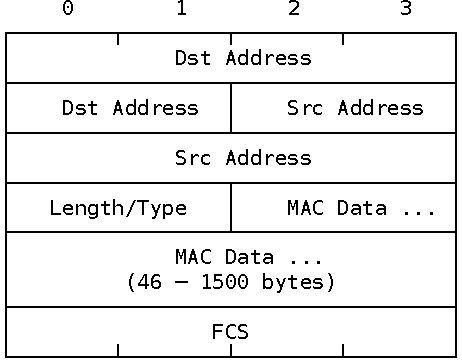
\includegraphics[width=.65\textwidth]{eth-frame}
      \caption{Ethernet Version II Frame Format}
      \label{fig:ethernet-frame-format}
    \end{figure}
  \end{frame}


  \subsubsection{ARP}

  \begin{frame}
    \frametitle{ARP}
    \begin{description}
    \item[ARP] Looking up the ARP table to find the destination MAC address.
    \end{description}    
    \begin{exampleblock}{Example ARP table}
      \begin{center}
        \begin{tabular}{|lr|}
          \hline
          IP address & Ethernet address\\\hline
          223.1.2.1  & 08-00-39-00-2F-C3\\
          223.1.2.3  & 08-00-5A-21-A7-22\\
          223.1.2.4  & 08-00-10-99-AC-54\\\hline
        \end{tabular}
      \end{center}
    \end{exampleblock}
  \end{frame}

  \begin{frame}
    \frametitle{ARP} \framesubtitle{Where does the ARP table come
      from?}
    \begin{exampleblock}{Example ARP Request}
      \begin{center}
        \begin{tabular}{|lr|}
        \hline
        Sender IP Address & 223.1.2.1\\
        Sender Enet Address & 08-00-39-00-2F-C3\\\hline
        Target IP Address & 223.1.2.2\\
        Target Enet Address & FF-FF-FF-FF-FF-FF\\\hline
      \end{tabular}
    \end{center}
    \end{exampleblock}

    \begin{exampleblock}{Example ARP Response}
      \begin{center}
        \begin{tabular}{|lr|}
          \hline
          Sender IP Address &  223.1.2.2\\
          Sender Enet Address & 08-00-28-00-38-A9\\\hline
          Target IP Address & 223.1.2.1\\
          Target Enet Address & 08-00-39-00-2F-C3\\\hline
        \end{tabular}
      \end{center}
    \end{exampleblock}
  \end{frame}
  
  \begin{frame}
    \frametitle{ARP} \framesubtitle{Where does the ARP table come from?}
    \begin{exampleblock}{The updated table}
      \begin{center}
        \begin{tabular}{|lr|}
          \hline
          IP address & Ethernet address\\\hline
          223.1.2.1 & 08-00-39-00-2F-C3\\
          223.1.2.2 & 08-00-28-00-38-A9\\
          223.1.2.3 & 08-00-5A-21-A7-22\\
          223.1.2.4 & 08-00-10-99-AC-54\\\hline
        \end{tabular}
      \end{center}
    \end{exampleblock}
  \end{frame}


  \subsubsection{IP}

  \begin{frame}
    \frametitle{IP} \framesubtitle{Router}
    \begin{figure}
      \centering
      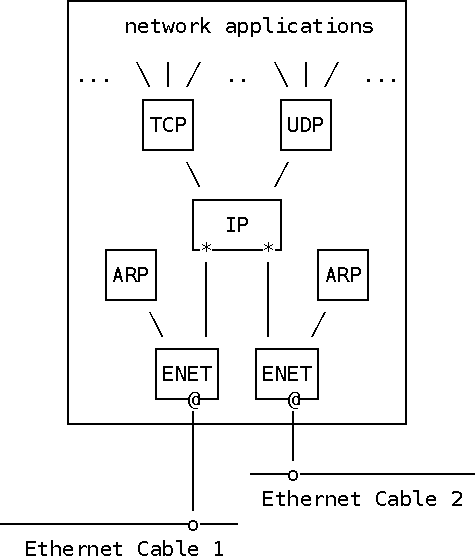
\includegraphics[width=.4\textwidth]{basic-structure-2}
      \caption{Router}
      \label{fig:router}
    \end{figure}
  \end{frame}

  \begin{frame}
    \frametitle{IP} \framesubtitle{Routing}
    \begin{description}
    \item[Routing] Find a route in the route table.
    \end{description}
  \end{frame}

  \begin{frame}
    \frametitle{IP} \framesubtitle{Direct Routing---IP is overhead}
    \begin{center}
      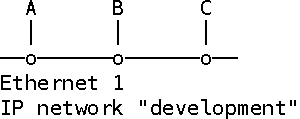
\includegraphics[height=.5\textheight]{direct-routing}
    \end{center}

    \begin{exampleblock}{Addresses in an Ethernet frame for an IP
        packet from A to B}
      \begin{center}
      \begin{tabular}{|lcc|}
        \hline
        address & source & destination\\\hline
        IP header & A & B\\
        Ethernet header & A & B\\\hline
      \end{tabular}
      \end{center}
    \end{exampleblock}
  \end{frame}

  \begin{frame}
    \frametitle{IP} \framesubtitle{Indirect Routing}
    \begin{figure}
      \centering
      \includegraphics[width=.9\textwidth]{indirect-routing}
      \caption{Three IP Networks; One Internet}
      \label{fig:indirect-routing}
    \end{figure}
    Computer D has a TCP/IP protocol stack similar to Figure~\ref{fig:router}.
  \end{frame}

  \begin{frame}
    \frametitle{IP} \framesubtitle{Indirect Routing}
    \begin{exampleblock}{Addresses in an Ethernet frame for an IP
        packet from A to E (before D)}
      \begin{center}
        \begin{tabular}{|lcc|}
          \hline
          address & source & destination\\\hline
          IP header & A & E \\
          Ethernet header & A & D \\\hline
        \end{tabular}
      \end{center}      
    \end{exampleblock}

    \begin{exampleblock}{Addresses in an Ethernet frame for an IP
        packet from A to E (after D)}
      \begin{center}
        \begin{tabular}{|lcc|}
          \hline
          address & source & destination\\\hline
          IP header & A & E \\
          Ethernet header & D & E \\\hline
        \end{tabular}
      \end{center}      
    \end{exampleblock}
  \end{frame}

  \begin{frame}
    \frametitle{IP} \framesubtitle{IP Module Routing Rules}
    \begin{enumerate}
    \item For an outgoing IP packet, entering IP from an upper layer,
      IP must decide whether to send the IP packet directly or
      indirectly, and IP must choose a lower network interface.  These
      choices are made by consulting the route table.
    \item For an incoming IP packet, entering IP from a lower
      interface, IP must decide whether to forward the IP packet or
      pass it to an upper layer.  If the IP packet is being forwarded,
      it is treated as an outgoing IP packet.
    \item When an incoming IP packet arrives it is never forwarded
      back out through the same network interface.
    \end{enumerate}    
  \end{frame}

  \begin{frame}
    \frametitle{IP} \framesubtitle{IP Address}
    \begin{exampleblock}{Address Formats}
      \begin{center}
        \begin{tabular}{|llcl|}
          \hline
          High & Format & Class & Decimal\\
          Order&&&Address\\
          Bits&&&Range\\\hline
          0 & 7 bits of net, & a & 1~126\\%$\sim{}doesn't work in xetex. Have to use Chinese ~$
          & 24 bits of host&&\\\hline
          10 & 14 bits of net, & b & 128~191\\
          & 16 bits of host&&\\\hline
          110 & 21 bits of net, & c & 192~223\\
          & 8 bits of host&&\\\hline
          111 & \multicolumn{3}{l|}{escape to extended addressing mode}\\\hline
        \end{tabular}
      \end{center}
    \end{exampleblock}
  \end{frame}

  \begin{frame}
    \frametitle{IP} \framesubtitle{Special IP Addresses}
    \begin{itemize}
    \item A value of zero in the network field means this
      network. (source only)
    \item A value of zero in the host field means network address.
    \item 127.x.x.x are loopback address.
    \item 255.255.255.255 is boardcast address.
    \item Private address:
      \begin{itemize}
      \item 10.x.x.x
      \item 172.16.x.x$\sim$172.31.x.x
      \item 192.168.x.x
      \end{itemize}
    \item CIDR---Classless Inter-Domain Routing---An IP addressing
      scheme that replaces the older system based on classes A, B and
      C. %(more in Section~\ref{sec:cidr})
    \end{itemize}
  \end{frame}

  \begin{frame}
    \frametitle{IP} \framesubtitle{Names}
    People refer to computers by names, not numbers.
    \begin{exampleblock}{/etc/hosts}
      \begin{center}
        \begin{tabular}{ll}
          127.0.0.1 & localhost\\
          202.203.132.242 & cs2.swfu.edu.cn\\
          & cs2
        \end{tabular}
      \end{center}
    \end{exampleblock}

    \begin{exampleblock}{/etc/networks}
      \begin{center}
        \begin{tabular}{ll}
          localnet & 202.203.132.192\\
        \end{tabular}
      \end{center}
    \end{exampleblock}
  \end{frame}

  \begin{frame}
    \frametitle{IP} \framesubtitle{IP Route Table}
    \begin{exampleblock}{Example IP Route Table}
      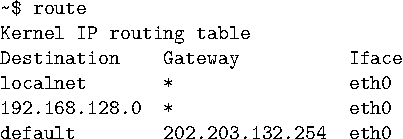
\includegraphics[width=\textwidth]{route-table}
    \end{exampleblock}
    'man route' for detailed meaning of each field.
  \end{frame}

  \begin{frame}
    \frametitle{IP} \framesubtitle{Direct Routing Details}
    \begin{center}
      \includegraphics[height=.55\textheight]{direct-routing-2}
    \end{center}

    \begin{exampleblock}{The route table inside alpha (simplified)}
      \begin{center}
        \begin{tabular}{|llcc|}
          \hline
          network & flag & router & interface\\\hline
          development & direct & & 1\\\hline
        \end{tabular}
      \end{center}
    \end{exampleblock}
  \end{frame}

  \begin{frame}
    \frametitle{IP} \framesubtitle{Direct Scenario}
    Alpha is sending an IP packet to beta...Please describe.
  \end{frame}
  
  \begin{frame}
    \frametitle{IP} \framesubtitle{Indirect Routing Details}\label{indirect-routing}
    \begin{center}
      \includegraphics[height=.75\textheight]{indirect-routing-2}
    \end{center}
    \tiny{(For protocol stack inside delta, see Figure~\ref{fig:router})}
  \end{frame}

  \begin{frame}
    \frametitle{IP} \framesubtitle{Indirect Routing Details}
    \begin{exampleblock}{The route table inside alpha}
      \begin{center}
        \begin{tabular}{|llcc|}
          \hline
          network & flag & router & interface\\\hline
          223.1.2 & direct & & 1\\
          223.1.3 & indirect & 223.1.2.4 & 1\\
          223.1.4 & indirect & 223.1.2.4 & 1\\\hline
        \end{tabular}
      \end{center}
    \end{exampleblock}

    \begin{exampleblock}{The route table inside delta}
      \begin{center}
        \begin{tabular}{|llcc|}
          \hline
          network & flag & router & interface \\\hline
          223.1.2 & direct & & 1\\
          223.1.3 & direct & & 3\\
          223.1.4 & direct & & 2\\\hline
        \end{tabular}
      \end{center}
    \end{exampleblock}
  \end{frame}

  \begin{frame}
    \frametitle{IP} \framesubtitle{Indirect Scenario}
    Alpha is sending an IP packet to epsilon...Please describe.
  \end{frame}

  \begin{frame}
    \frametitle{IP} \framesubtitle{Managing The Routes}
    \begin{itemize}
    \item Manually maintained by administrator
    \item ICMP can report some routing problems
    \item For larger networks, routing protocols are used.
    \end{itemize}
  \end{frame}

  \begin{frame}
    \frametitle{IP Packet}
    \begin{figure}
      \centering
      \includegraphics[width=\textwidth]{ip-packet}
      \caption{IP Packet Format}
      \label{fig:ip-packet-format}
    \end{figure}
  \end{frame}

  \subsubsection{Network Devices}

  \begin{frame} \frametitle{Networking Devices}
    \includegraphics[width=\textwidth]{net_devs}
  \end{frame}
  
%  \subsection{Repeater, Hub}
  
  \begin{frame} \frametitle{Physical Layer Networking Devices}
    \begin{description}
    \item[Repeater] connects network segments at the physical layer.\pause
    \item[Hub] a multi-port repeater \pause
    \end{description}
    \begin{itemize}
    \item simple, cheap
    \item Repeaters/Hubs do NOT isolate collision domains.
    \item 100m maximum
    \end{itemize}    
  \end{frame}
  
%  \subsection{Bridge, Switch}
  
  \begin{frame} \frametitle{Link Layer Networking Devices}
    \begin{description}
    \item[Bridge] connects multiple network segments at the data link layer (layer 2)
    \item[Switch] a multi-port bridge
    \end{description}
    \begin{exampleblock}{Transparent bridging}
      Uses a forwarding database to send frames across network segments
      \begin{itemize}
      \item Learning
      \item Flooding
      \item Forwarding
      \item Filtering
      \item Aging
      \end{itemize}
    \end{exampleblock}
  \end{frame}
  
 % \subsection{router}
  \begin{frame} \frametitle{Network Layer Networking Devices}
    \begin{description}
    \item[Router] connects two or more logical subnets at the network
      layer (layer 3)
    \item[Routing] is to find a route in the route table.(page \ref{indirect-routing})
    \end{description}
    \begin{exampleblock}{Bridging vs. Routing}
      \begin{center}
        \begin{tabular}{r|l}
          L2&L3\\\hline
          MAC addr.(local)&IP addr.(global)\\\hline
          intranet&internet\\\hline
          Forwarding DB&Routing table\\\hline
          relearn, flooding&more efficient
        \end{tabular}
      \end{center}
    \end{exampleblock}
    \begin{itemize}
    \item to put multiple segments into one bridged network, or
    \item to divide it into different networks interconnected by routers
    \end{itemize}
  \end{frame}
  
  %% \subsubsection{TCP}

  %% \begin{frame} \frametitle{TCP Summary}
  %%   \begin{itemize}
  %%   \item Stream data transfer
  %%   \item Reliability
  %%   \item Flow control
  %%   \item Multiplexing
  %%   \item Logical Connections
  %%   \item Full Duplex
  %%   \end{itemize}
  %% \end{frame}

  %% \begin{frame} \frametitle{TCP}\framesubtitle{Stream Data Transfer}
  %%   From the application's viewpoint, TCP transfers a contiguous
  %%   stream of bytes. TCP does this by grouping the bytes in TCP
  %%   segments, which are passed to IP for transmission to the
  %%   destination. TCP itself decides how to segment the data and it may
  %%   forward the data at its own convenience.
  %% \end{frame}

  %% \begin{frame} \frametitle{TCP}\framesubtitle{Reliability} TCP
  %%   assigns a sequence number to each byte transmitted, and expects a
  %%   positive acknowledgment (ACK) from the receiving TCP. If the ACK
  %%   is not received within a timeout interval, the data is
  %%   retransmitted. The receiving TCP uses the sequence numbers to
  %%   rearrange the segments when they arrive out of order, and to
  %%   eliminate duplicate segments.
  %% \end{frame}

  %% \begin{frame} \frametitle{TCP}\framesubtitle{Flow Control} The
  %%   receiving TCP, when sending an ACK back to the sender, also
  %%   indicates to the sender the number of bytes it can receive beyond
  %%   the last received TCP segment, without causing overrun and
  %%   overflow in its internal buffers. This is sent in the ACK in the
  %%   form of the highest sequence number it can receive without
  %%   problems.
  %% \end{frame}

  %% \begin{frame} \frametitle{TCP}\framesubtitle{Multiplexing} To allow
  %%   for many processes within a single host to use TCP communication
  %%   facilities simultaneously, the TCP provides a set of addresses or
  %%   ports within each host. Concatenated with the network and host
  %%   addresses from the internet communication layer, this forms a
  %%   socket. A pair of sockets uniquely identifies each connection.
  %% \end{frame}

  %% \begin{frame} \frametitle{TCP}\framesubtitle{Logical Connection} The
  %%   reliability and flow control mechanisms described above require
  %%   that TCP initializes and maintains certain status information for
  %%   each data stream. The combination of this status, including
  %%   sockets, sequence numbers and window sizes, is called a logical
  %%   connection.  Each connection is uniquely identified by the pair of
  %%   sockets used by the sending and receiving processes.
  %% \end{frame}

  %% \begin{frame} \frametitle{TCP}\framesubtitle{Full Duplex} TCP
  %%   provides for concurrent data streams in both directions.
  %% \end{frame}

  %% \begin{frame}
  %%   \frametitle{TCP Segment}
  %%   \begin{figure}
  %%     \centering
  %%     \includegraphics[width=.85\textwidth]{tcp-segment}
  %%     \caption{TCP Segment Format}
  %%     \label{fig:tcp-segment-format}
  %%   \end{figure}
  %% \end{frame}

  %% \begin{frame}[plain] \frametitle{State Transition Diagram}
  %%   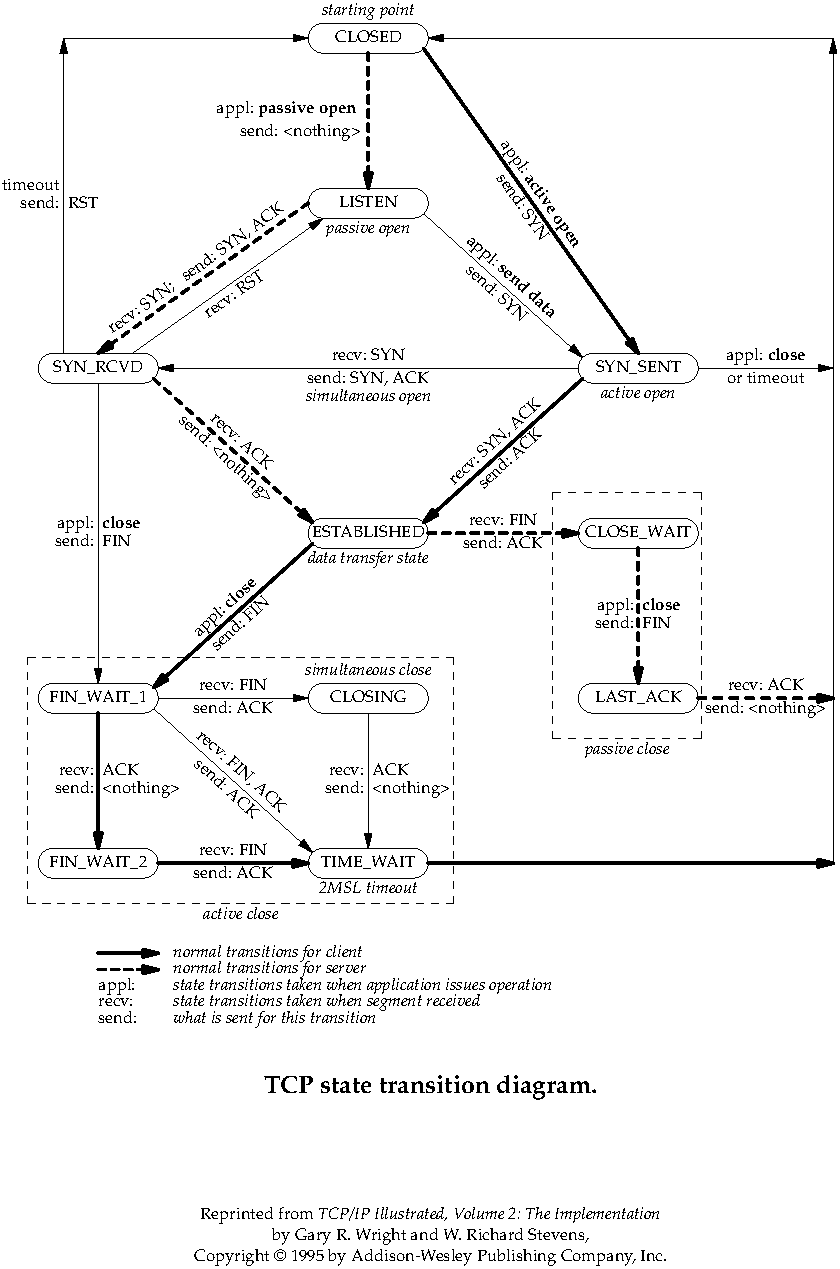
\includegraphics[height=1.65\textheight]{state_stevens}
  %% \end{frame}

  %% \begin{frame} \frametitle{Sliding Window}
  %%   \begin{center}
  %%     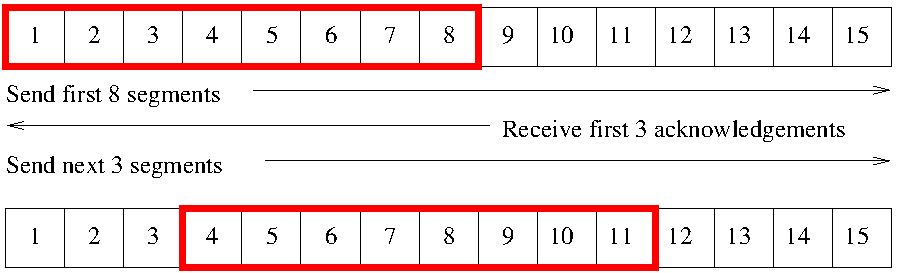
\includegraphics[width=\textwidth]{sliding_window}
  %%   \end{center}
  %%   \begin{exampleblock}{The sliding window serves several purposes:}
  %%     \begin{itemize}
  %%     \item it guarantees the reliable delivery of data
  %%     \item it ensures that the data is delivered in order
  %%     \item it enforces flow control between the sender and the
  %%       receiver.
  %%     \end{itemize}
  %%   \end{exampleblock}
  %% \end{frame}
  
  %% \subsection{UDP}

  %% \begin{frame}
  %%   \frametitle{UDP Datagram}
  %%   \begin{figure}
  %%     \centering
  %%     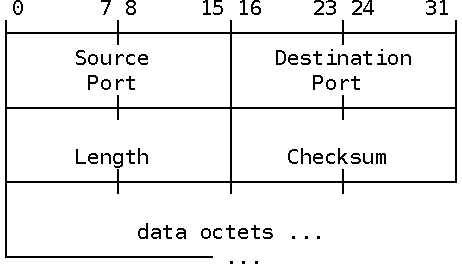
\includegraphics[width=.9\textwidth]{udp-datagram}
  %%     \caption{UDP Datagram Format}
  %%     \label{fig:udp-datagram-format}
  %%   \end{figure}
  %% \end{frame}

  %% \subsection{Network Applications}

  %% \begin{frame}
  %%   \frametitle{Application Layer}
  %%   Telnet, FTP, SNMP, SMTP, HTTP...
  %% \end{frame}


%% \subsection{How an Email is Delivered?}
%% \label{sec:how}


\section[Google]{The Logo of The Internet}
\label{sec:google}

% \begin{frame}\frametitle{}
% \small{\tableofcontents[currentsection]}
% \end{frame}

\begin{frame}\frametitle{The Logo of The Internet}
What pops up in your mind if I say ``Internet''?
\end{frame}

\subsection[Why Google?]{Google Philosophy}
\label{sec:why}

\begin{frame}\frametitle{\googlelogo{} Philosophy}
\framesubtitle{\href{http://www.google.com/corporate/tenthings.html}{Ten things Google has found to be true}}

\begin{enumerate}
\item Focus on the user and all else will follow.
\item It's best to do one thing really, really well.
\item Fast is better than slow.
\item Democracy on the web works.
\item You don't need to be at your desk to need an answer.
\item You can make money without doing evil.
\item There's always more information out there.
\item The need for information crosses all borders.
\item You can be serious without a suit.
\item Great just isn't good enough.
\end{enumerate}

\end{frame}

\begin{frame}\frametitle{\googlelogo{} Philosophy}\framesubtitle{\href{http://www.google.com/corporate/software_principles.html}{Software Principles}}                                                                 

\begin{enumerate}
\item  INSTALLATION --- We believe software should not trick you into installing it.
\item UPFRONT DISCLOSURE --- When an application is installed or enabled, it should inform you of its principal and significant functions.
\item SIMPLE REMOVAL --- It should be easy for you to figure out how to disable or delete an application.
\item CLEAR BEHAVIOR --- Applications that affect or change your user experience should make clear they are the reason for those changes.
\item SNOOPING --- If an application collects or transmits your personal information such as your address, you should know.
\item KEEPING GOOD COMPANY --- Application providers should not allow their products to be bundled with applications that do not meet these guidelines.
\end{enumerate}

\end{frame}


\begin{frame}\frametitle{\googlelogo{} Philosophy}
\framesubtitle{\href{http://www.google.com/corporate/ux.html}{Google User Experience}}

\begin{enumerate}
\item Focus on people – their lives, their work, their dreams. 
\item Every millisecond counts. 
\item Simplicity is powerful.
\item Engage beginners and attract experts.
\item Dare to innovate.
\item Design for the world.
\item Plan for today's and tomorrow's business.
\item Delight the eye without distracting the mind.
\item Be worthy of people's trust.
\item Add a human touch.
\end{enumerate}

\end{frame}

\begin{frame}\frametitle{\googlelogo{} Philosophy}
\framesubtitle{\href{http://www.google.com/corporate/nopopupads.html}{No pop-ups}}
We do not allow pop-up ads of any kind on our site.
\end{frame}

\begin{frame}\frametitle{\googlelogo{} Philosophy}
\framesubtitle{\href{http://www.google.com/corporate/security.html}{Security} }

\begin{itemize}
\item Google Security 
\item Product Safety
\end{itemize}

\end{frame}


\subsection{Google Products}
\label{sec:product}

\begin{frame}\frametitle{\googlelogo{} Products}

\begin{center}
  \href{http://www.google.com}{\includegraphics[height=1em]{gsearch}}
  \href{http://gmail.com}{\includegraphics[height=1em]{gmail}}
  \href{http://www.google.com/calendar/}{\includegraphics[height=1em]{gcalendar}}
  \href{http://reader.google.com}{\includegraphics[height=1em]{greader}}
  \href{http://docs.google.com/}{\includegraphics[height=1em]{gdocs}}
  \href{http://picasaweb.google.com}{\includegraphics[height=1em]{gpicasa}}
  \href{http://www.google.com/finance}{\includegraphics[height=1em]{gfinance}}
  \href{http://www.google.cn/ig}{\includegraphics[height=1em]{igoogle}}
  \href{http://maps.google.com}{\includegraphics[height=1em]{gmaps}}
  \href{http://earth.google.com}{\includegraphics[height=1em]{gearth}}
  \href{http://sketchup.google.com}{\includegraphics[height=1em]{gsketchup}}
  \href{http://www.google.cn/music}{\includegraphics[height=1em]{gmusic}}
  \href{http://translate.google.cn}{\includegraphics[height=1em]{gtranslate}}
  \href{http://tools.google.com/pinyin}{\includegraphics[height=1em]{gime}}
  \href{http://www.google.com/chrome}{
\includegraphics[height=1em]{gchrome}}
\end{center}

\begin{center}
  \href{http://www.google.cn/intl/zh-CN/options/}{a lot more...}
\end{center}

\end{frame}

\section{Safe Surfing}
\label{sec:safe}

% \begin{frame}\frametitle{}
% \small{\tableofcontents[currentsection]}
% \end{frame}

\subsection[Dangerous]{Viruses, Worms, Trojan Horses, Malware, Adware, and Spyware}
\label{sec:virus}

\begin{frame}\frametitle{Viruses, Worms, and Trojan Horses}

\begin{description}
\item[A computer virus] is a computer program that can copy itself and infect a computer without the permission or knowledge of the owner.
\item[A computer worm] is a self-replicating computer program. It uses a network to send copies of itself to other nodes (computers on the network) and it may do so without any user intervention. Unlike a virus, it does not need to attach itself to an existing program.
\item[A Trojan horse,] or \emph{trojan} for short, is a term used to describe malware that appears, to the user, to perform a desirable function but, in fact, facilitates unauthorized access to the user's computer system. Trojan horses are not self-replicating which distinguishes them from viruses and worms. 
\end{description}

\end{frame}

\begin{frame}\frametitle{Malware, Adware, and Spyware}

\begin{description}
\item[Malware,] short for malicious software, is software designed to infiltrate or damage a computer system without the
  owner's informed consent. Malware includes computer viruses, worms, trojan horses, most rootkits, spyware, dishonest
  adware, crimeware ...
\item[Adware] or advertising-supported software is any software package which automatically plays, displays, or downloads advertisements to a computer after the software is installed on it or while the application is being used. Some types of adware are also spyware and can be classified as privacy-invasive software.
\item[Spyware] is a type of malware that is installed on computers and that collects information about users without their knowledge.
\end{description}

\end{frame}

\subsection[Browsers]{Choose The Right Tool To Do The Right Thing}
\label{sec:tools}

\begin{frame}\frametitle{Choose The Right Tool To Do The Right Thing}

\begin{center}
\begin{tabular}{ccc}
  
\includegraphics[height=5em]{windows}&\includegraphics[height=5em]{linuxlogo}&\includegraphics[height=5em]{applelogo}\\
  \includegraphics[height=5em]{ie}&\includegraphics[height=5em]{firefox}&\includegraphics[height=5em]{gchrome}
\end{tabular}
\end{center}

\begin{center}
\begin{Huge}
\googlelogo{} ~\href{http://www.google.com/search?q=google+vs+baidu&ie=utf-8&oe=utf-8&aq=t&rls=org.debian:en-US:unofficial&client=iceweasel-a}{vs.}~\includegraphics[height=1.2em]{baidu}
\end{Huge}
\end{center}             

\end{frame}

\subsection[Advices]{Safe Surfing Advice}
\label{sec:advice}

\begin{frame}\frametitle{Safe Surfing Advice}\framesubtitle{Take care of your identity and privacy}

\begin{itemize}
\item Avoid identity theft by using an up to date web browser and blocking bogus emails with a spam filter
\item Always use strong passwords
\item Don’t give away too much personal information on blogs and social networking sites
\end{itemize}

\end{frame}

\begin{frame}\frametitle{Safe Surfing Advice}\framesubtitle{Protect Your PC}

\begin{itemize}
\item Get anti-virus software, anti-spyware software and a firewall
\item Keep your computer up to date
\item Block spam emails
\item Use an up to date web browser
\item Make regular backups
\item Encrypt your wireless network
\end{itemize}

\end{frame}

\begin{frame}\frametitle{Safe Surfing Advice}\framesubtitle{Avoid online rip-offs}

\begin{itemize}
\item When you’re shopping online, look for clear signs that you’re buying from a reputable company
\item On an online auction site, learn how it works and learn to pick good sellers
\item Use safe ways to pay, such as PayPal or credit and debit cards
\item Use your common sense to avoid scams – if it sounds too good to be true, it probably is
\end{itemize}

\end{frame}

\begin{frame}\frametitle{Recommended Websites}

\begin{itemize}
\item \href{http://google.com}{Google}
\item \href{http://en.wikipedia.org}{Wikipedia}
\item \href{http://del.icio.us}{Delicious}
\item \href{http://ocw.mit.edu/OcwWeb/web/home/home/index.htm}{MIT Open Courseware}      
\item \href{http://www.librivox.org}{Librivox}      
\end{itemize}

\end{frame}

\begin{frame}\frametitle{References}

\begin{thebibliography}{}
\bibitem[RFC1180]{}\href{http://www.rfc-editor.org/rfc/rfc1180.txt}{RFC1180 - TCP/IP tutorial}
\bibitem[RFC1122]{}\href{http://www.faqs.org/rfcs/rfc1122.html}{RFC1122 - Requirements for Internet Hosts - Communication Layers}
\bibitem[RFC1123]{}\href{http://www.faqs.org/rfcs/rfc1123.html}{RFC 1123 - Requirements for Internet Hosts - Application and Support}                   
\bibitem[RFC791]{}\href{http://www.ietf.org/rfc/rfc791.txt}{RFC791 - Internet Protocol}
\bibitem[RFC2235]{}\href{http://www.faqs.org/rfcs/rfc2235.html}{RFC2235 - Hobbes' Internet Timeline}
\bibitem[]{}\href{http://en.wikipedia.org/wiki/Computer_network}{Wikipedia - Computer Network}
\bibitem[]{}\href{http://en.wikipedia.org/wiki/Computer_virus}{Wikipedia - Computer Virus}
\bibitem[]{}\href{http://www.google.com/intl/en/corporate/}{\googlelogo{} Corporate Information}
\end{thebibliography}

\end{frame}

\end{document}
